\documentclass[10pt,a4paper]{article}
\usepackage[utf8]{inputenc}

\usepackage{amsmath}
\usepackage{amsfonts}
\usepackage{amssymb}
\usepackage{graphicx}
\usepackage{listings}
\usepackage{refstyle}
\usepackage{wasysym}
\usepackage{subfigure}

\lstset{numbers=left,
	title=\lstname,
	numberstyle=\tiny, 
	breaklines=true,
	tabsize=4,
	language=Python,
	morekeywords={with,super,as},,
	frame=single,
	basicstyle=\footnotesize\tt,
	commentstyle=\color{comment},
	keywordstyle=\color{keyword},
	stringstyle=\color{string},
	backgroundcolor=\color{white},
	showstringspaces=false,
	numbers=left,
	numbersep=5pt,
	literate=
		{æ}{{\ae}}1
		{å}{{\aa}}1
		{ø}{{\o}}1
		{Æ}{{\AE}}1
		{Å}{{\AA}}1
		{Ø}{{\O}}1
	}

\usepackage{bm}
\usepackage{hyperref}
\usepackage{xcolor}
%Denne seksjonen under sørger for at linken blir blå og ikke rød.
\hypersetup{                
    colorlinks,
    linkcolor={black},
    citecolor={blue!50!black},
    urlcolor={blue!80!black}
}
\urlstyle{same}

\usepackage[margin=1.25 in]{geometry}
%\usepackage[usenames, dvipsnames]{color}
\usepackage{float}
\usepackage{commath}

\begin{document}
\begin{center}

{\LARGE\bf
FYS4150\\
\vspace{0.5cm}
Project 5, deadline December 10.
}
 
\includegraphics[scale=0.075]{figures/uio.png}\\
Authors: Robin David Kifle, Sander Wågønes Losnedahl, Sigmund Slang and Vemund Stenbekk Thorkildsen\\
\vspace{1cm}
{\LARGE\bf
Abstract
}\\
\end{center}
We have developed a program to simulate temperature distribution and development. This has been done using three different algorithms. Namely the Euler forward, Euler backward and the Crank-nicolson schemes. All the algorithms have different advantages and drawbacks. For instance, the Euler forward scheme is efficient and easy to implement, but can be unstable for unfavorable step sizes. We used these algorithms to evaluate three models. The first being the temperature distribution in a simple one dimensional rod. This was evaluated by simulating the temperature with all three schemes. When moving to the second model, an idealized two dimensional system with a heat source in one end, we had to decide what kind of boundary conditions we wanted to use. We decide to simulated the model with both periodic boundary conditions and hard coded zero temperature at three edges. This leads to two entirely different results. The third model consists of three layers, each with different heat production constants. This was first modeled with the initial parameters, and the second with an extra heat production in the bottom layer. This additional heat production is made by radioactive materials, and alters the temperature distribution throughout the model. The temperature is generally higher, and the distribution is non-linear, which is in clear contrast to the approximately linear distribution seen without enrichment. It was decided to use the Euler forward scheme for both the two dimensional models. As we needed to simulate over a long time span, a lot of the constants had to be scaled up. This had to be done as to avoid unstable results. It is hard to determine which of the schemes is best, as this is entirely decided by what kind of problem you want to simulate, but for this case it was ultimately the ease of implementation and computational efficiency that made us choose the Euler forward scheme for the two dimensional case. 

\newpage
\section*{Introduction}
The aim of this project is to use three different finite difference schemes to simulate temperature variations for three different models. The three schemes are the implicit Euler backward, explicit Euler forward and the Crank-Nicolson scheme. This is a combination of the Euler forward and backward schemes. These schemes can be used to simulate a variety of physical phenomena, but for simplicity will here be discussed in terms of temperature only.\\ 

\noindent The first part will mostly revolve around idealized situations in one dimension, before moving on to an idealized two dimensional problem. This is followed by a three layered model of the earths crust, where each has different parameters of heat production. The three layered model will be simulated two times. Once for initial heat production parameters, and once where the heat production of the bottom layer (mantle) is increased by just over an order of magnitude. All the code, runs and figures for the project is accessible \href{https://github.com/VemundStenbekkThorkildsen/Assignment5}{\textcolor{blue}{here}}.  



\section*{Method}

\noindent The three different schemes are differential equations that can be rewritten as a set of linear equations. The Euler forward is explicit, the Euler backward is implicit, while the Crank-Nicolson scheme is a combination of the two preceding schemes. These systems can be rewritten as sets of linear equations. \\


\noindent The Euler backwards scheme is implicit, as it uses the current step $i$, to derive the previous step $i-1$. 
\\
\begin{equation}
u_t \approx \frac{u(x_i,t_j) - u(x_i,t_j - \Delta t)}{\Delta t}
\end{equation}

\begin{equation}
u_{xx} \approx \frac{u(x_i + \Delta x,t_j) - 2u(x_i,t_j) + u(x_i - \Delta x,t_j)}{\Delta x^2}
\end{equation}

\noindent It is possible to scale the above equation by $\alpha = \Delta t / \Delta x^2$, so the equation only depends on one scaled variable. This leads to:

\begin{equation}
u_{i,j-1} = -\alpha u_{i-1,j} + (1 + 2\alpha)u_{i,j} - \alpha u_{i+1,j}
\end{equation}

\noindent Now the differential equation can be written as a set of linear equations with a matrix $A$ times a vector $V_j$ such that $AV_j = V_{j-1}$. Where $A$, defined from the above differential equations take the form:

\begin{equation}
A = \begin{bmatrix}
1 + 2\alpha & -\alpha & 0 & 0 &\cdots\\
-\alpha & 1 + 2\alpha & -\alpha & 0 & \cdots\\
\cdots & \cdots & \cdots & \cdots & \cdots\\
0 & 0 & \cdots & -\alpha & 1 + 2\alpha\\

\end{bmatrix}
\end{equation}

\noindent It is now possible to find the previous vector $V_{j-1}$ when $V_j$ is known.This means that it is essential to have initial conditions to start the calculations. A more generalized equation can be written as:

\begin{equation}
A^{-1}(AV_j) = A^{-1}(V_{j-1})
\end{equation}
\noindent By continuing to multiply by $A^{-1}$, the implicit scheme takes the form:

\begin{equation}
V_j = A^{-j}V_0
\end{equation}

\noindent A very similar process can be applied to the Euler forward method, but this scheme is explicit:

\begin{equation}
u_t = \frac{u(x_i,t_j + \Delta t) - u(x_i,t_j)}{\Delta t}
\end{equation}

\begin{equation}
u_{xx} \approx \frac{u(x_i + \Delta x,t_j) - 2u(x_i,t_j) + u(x_i - \Delta x,t_j)}{\Delta x^2} 
\end{equation}

\begin{equation}
u_{i,j-1} = \alpha u_{i-1,j} + (1 - 2\alpha)u_{i,j} + \alpha u_{i+1,j}
\end{equation}

\begin{equation}
A = \begin{bmatrix}
1 - 2\alpha & \alpha & 0 & 0 &\cdots\\
\alpha & 1 - 2\alpha & \alpha & 0 & \cdots\\
\cdots & \cdots & \cdots & \cdots & \cdots\\
0 & 0 & \cdots & \alpha & 1 - 2\alpha\\

\end{bmatrix}
\end{equation}

\noindent such that:

\begin{equation}
V_{j+1} = AVj
\end{equation}

\noindent Generalizing again and get:

\begin{equation}
V_{j+1}= A^{j+1}V_{0}
\end{equation}

\noindent The Crank-Nicolson scheme is is a combination of both the implicit Euler backward and explicit Euler forward scheme.

\begin{equation}
\frac{\theta}{\Delta x^2}(u_{i-1,j} - 2u_{i,j} + u_{i+1,j}) + \frac{1 - \theta}{\Delta x^2}(u_{i+1,j-1} - 2u_{i,j-1} + u_{i-1,j-1}) = \frac{1}{\Delta t}(u_{i,j} - u_{i,j-1})
\end{equation}

\noindent Where $\theta$ determines whether the scheme is explicit when $\theta = 0$, or implicit when $\theta = 1$. However, to get the actual Crank-Nicolson scheme, it is required to have $\theta = 1/2$. This is stable for all $\Delta x$ and $\Delta t$. The Crank-Nicolson scheme is derived by Taylor expanding the forward Euler method $u(x,t + \Delta t)$, $u(x + \Delta x,t)$, $u(x - \Delta x,t)$, $u(x + \Delta x, t + \Delta t)$ and $u(x + \Delta x, t + \Delta t)$ for $t + \Delta t/2$.\\

\noindent Scaling the equation with $\alpha = \frac{\Delta t}{\Delta x^2}$ gives the following equation:

\begin{equation}
-\alpha u_{i-1,j} + (2 + 2\alpha)u_{i,j} -\alpha u_{i+1,j} = \alpha u_{i-1,j-1} + (2-2\alpha)u_{i,j-1} + \alpha u_{i+1,j-1}
\end{equation}

\noindent which can be rewritten as

\begin{equation}
(2I + \alpha B)V_j = (2I - \alpha B)V_{j-1}
\end{equation}

\begin{equation}
V_j = (2I + \alpha B)^{-1}(2I - \alpha B)V_{j-1}
\end{equation}

\noindent where I is the identity matrix and B is given by:

\begin{equation}
B = \begin{bmatrix}
2 & -1 & 0 & \cdots &0\\
-1 & 2 & -1 & 0 & \vdots\\
\vdots & \ddots & \ddots & \ddots & \vdots\\
\vdots & 0 & \ddots & \ddots & -1\\
0 & \cdots & \cdots & -1 & 2\\
\end{bmatrix}
\end{equation}


\noindent The analytic solution for the one dimensional at equilibrium can be solved by using:


\begin{equation} 
t\rightarrow\infty \hspace{1cm} \Rightarrow \hspace{1cm}u_t=0
\end{equation}

\noindent This makes Laplaces' equation $\nabla^2u=0$. In one dimension this translates to $u_{xx}=0$. By integrating once: $u_x=c_1$, integrating twice: $u_{xx}=c_1x+c_2$. Using the boundary conditions $u(0)=0$ and $u(1)=1$ makes:

\begin{equation}
u(0)=0\rightarrow c_2=0
\end{equation}

\begin{equation}
u(1)=1 \rightarrow c_1=1
\end{equation}
which gives:
\begin{equation}
\rightarrow u(x,t)_{t\rightarrow\infty}=x
\end{equation}
\noindent In other words, a linear graph. The solution for two dimensions is somewhat harder to solve, but starts in the same manner. That is:\\

\begin{equation}
\nabla^2_{t\rightarrow \infty}=0 \hspace{0.5cm} \rightarrow \hspace{0.5cm} u_{xx}+u_{yy}=0
\end{equation}

\noindent Ansatz: $u(x,y)=F(x)G(y)$, giving the double derivative: 

\begin{equation}
u''(x,y)=F_{xx}G+FG_{yy}=0 \rightarrow \frac{F_{xx}}{F}=-\frac{G_{yy}}{G}
\end{equation}

\noindent This needs to be equal to a constant $\lambda$. Because of the given boundaries, $G(y)$ has to equal $sin(\sqrt{\lambda}y)$. The boundaries $G(0)=0$ and $G(H=1)=0$ gives $\lambda=(n\pi)^2$\\

\noindent Now, by looking at $F_{xx}=\lambda F$ and making a new ansatz: 

\begin{equation}
F(x)=Ae^{(n\pi x)}+Be^{-(n\pi x)}
\end{equation}

\noindent and looking boundary $F(0)=0$ gives $B=-A$. Which in turn gives the expression for 

\begin{equation}
F(x) \rightarrow F(x)=Asinh(n\pi x)
\end{equation}

\noindent Giving the solution $u(x,y)=F(x)G(x)$:\\

\begin{equation}
u(x,y)=\sum^\infty_{n=1}A_nsinh(n\pi x)sin(n\pi y)
\end{equation}

\noindent By then using the last boundary, $u(1,y)=1$, to find an expression for $A_n$ by taking the integral of both sides: 


\begin{equation}
\int_0^1 1*sin(m\pi y) dy = \int_0^1 \sum^\infty_{n=1}A_nsinh(n\pi 1)sin(n\pi y)*sin(m\pi y)
\end{equation}

\noindent For $n\neq m$, the integral on the right is equal to 0. Because of this the integral can be written as:


\begin{equation}
int_0^1 1*sin(n\pi y) dy = \int_0^1 \sum^\infty_{n=1}A_nsinh(n\pi 1)2sin(n\pi y)
\end{equation}

\begin{equation}
= \frac{A_n}{2}sinh(n\pi) 
\end{equation}

\noindent Giving an equation that can be solved for $A_n$:\\

\begin{equation}
\frac{2}{sinh(n\pi)}\int_0^1sin(n\pi y) dy
\end{equation}

The integral has solutions for odd $n = \frac{2}{n\pi}$, and even $n = 0$. Now the problem can be solved analytically. The correct solution is given by letting $n \rightarrow \infty$, but a good approximation can be found by letting $n$ run from $0$ to $100$. 










\noindent The analytic solution for the three layer model in one dimension can be solved by considering the heat equation at equilibrium:\\

\begin{equation}
\nabla(k\nabla T) +Q=\rho c_p \frac{\partial T}{\partial t} \Rightarrow \frac{\partial T}{\partial t}=0
\end{equation}

\noindent By integrating two times over z, this equals:
\begin{equation}
a=-\frac{Q_n}{2K}
\end{equation}
\begin{equation}
\frac{\partial T_n}{\partial z}=2a_nz+b_n
\end{equation}
\begin{equation}
T_n=a_nz^2+b_nz+c_n \hspace{0.5cm} n= 1,2,3
\end{equation}

\noindent The temperature and heat flow is continuous at the boundaries, which is located at z=0, z=-20 and z=-40:\\

\noindent Heat flow:
\begin{equation}
\frac{ \partial T_1(-20)}{\partial z}=\frac{\partial T_2(-20)}{\partial z},
\frac{\partial T_2(-40)}{\partial z}=\frac{\partial T_3(-40)}{\partial z}
\end{equation}

\noindent Temperature:
\begin{equation}
T_1(0)=8 \rightarrow c_1=8 \hspace{1cm}
T_1(-20)=T_2(-20) \hspace{1cm}
T_2(-40)=T_2(-40)
\end{equation}




\noindent These conditions make it possible to express $b_1$ and $b_2$, by $b_3$:\\

\begin{equation}
b=\begin{bmatrix}
-6+b_3\\
2.4+b_3\\
b_3\\
\end{bmatrix}
\end{equation}

\noindent These relations have been used to find $b-$ and $c$-values.






\section*{Implementation}

\noindent The implicit Euler scheme were first implemented due to its simplicity, not needing any tri-diagonal solvers. However, this simplicity comes on the cost of stability which can be seen in Table \ref{truncstab}. Next, the explicit schemes were implemented, as well as the LU triangular solver which is the backbone for the explicit Euler scheme. Crank-Nicolson does not solely rely on the LU solver, but has an implicit component as well.\\

\noindent Only the implicit scheme were extended to an additional dimension. Again, this is for the sake of simplicity, but one has to be aware of the stability requirements.
\\
When the code is extended an additional dimension, the boundary conditions have to be extended accordingly. A problem arises at the edges of the two-dimensional grid where no boundary conditions exists, because the implicit scheme needs four adjacent points to calculate the current point, but at the edges there are only three available points. To resolve this issue, one has to use the point at the opposite edge.
\\
To solve the geological case, the implicit scheme has to be adjusted with the $1300 C^{\circ}$ at the bottom of the lithosphere and $8 C^{\circ}$ at the top of the crust. Additionally, there is heat production at at certain ranges which were also implemented.



\newpage
\section*{Results}


\noindent The truncation errors and stability is calculated in the Taylor expansion and these values are shown in the table below:


\begin{table}[H]
\centering
\caption{Truncation errors and stability for the three methods}
\begin{tabular}{|c|c|c|}
\hline
Method & Truncation error & Stability for\\
\hline
Euler Forward & $\Delta x^2$, $\Delta t$ & $\frac{1}{2} \Delta x^2 \geq \Delta t$\\
\hline
Euler Backward & $\Delta x^2$, $\Delta t$ & $\Delta x^2$ and $\Delta t^2$\\
\hline
Crank-Nicolson & $\Delta x^2$, $\Delta t^2$ & $\Delta x^2$ and $\Delta t^2$\\
\hline
\end{tabular}
\label{truncstab}
\end{table}
 

\noindent Table \ref{truncstab} shows that the Euler backward and Crank-nicolson schemes have no limitations for $\Delta x$ and $\Delta t$. 


\begin{figure}[H]
 	\centering
  	\subfigure[\ $t_1$]{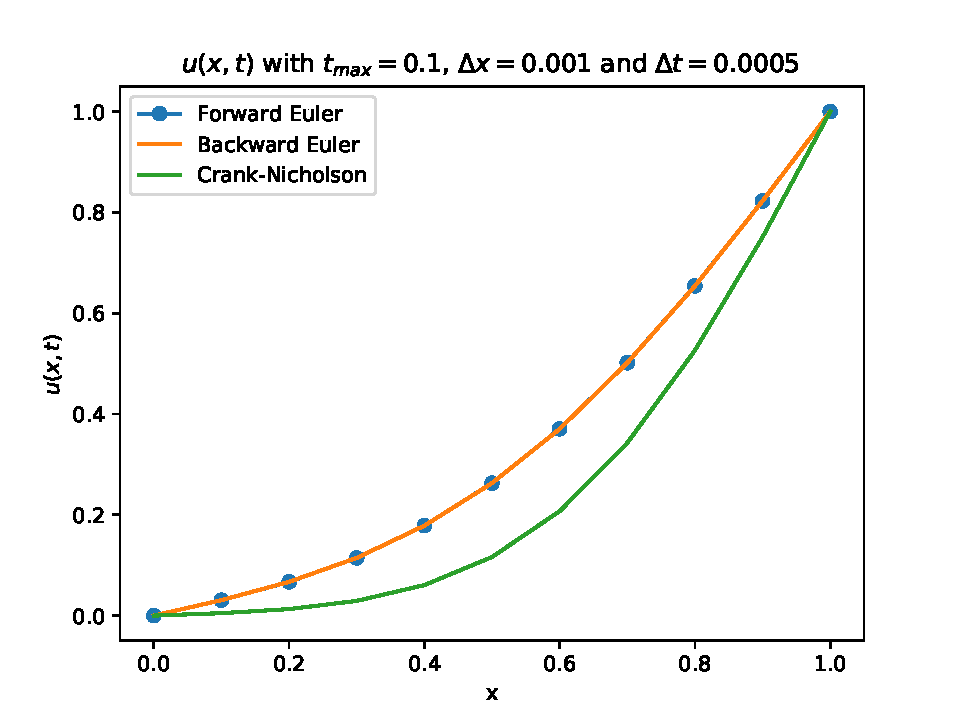
\includegraphics[width = 0.49\textwidth]{../plots/t1_10.pdf}}  
  	\subfigure[\ $t_2$]{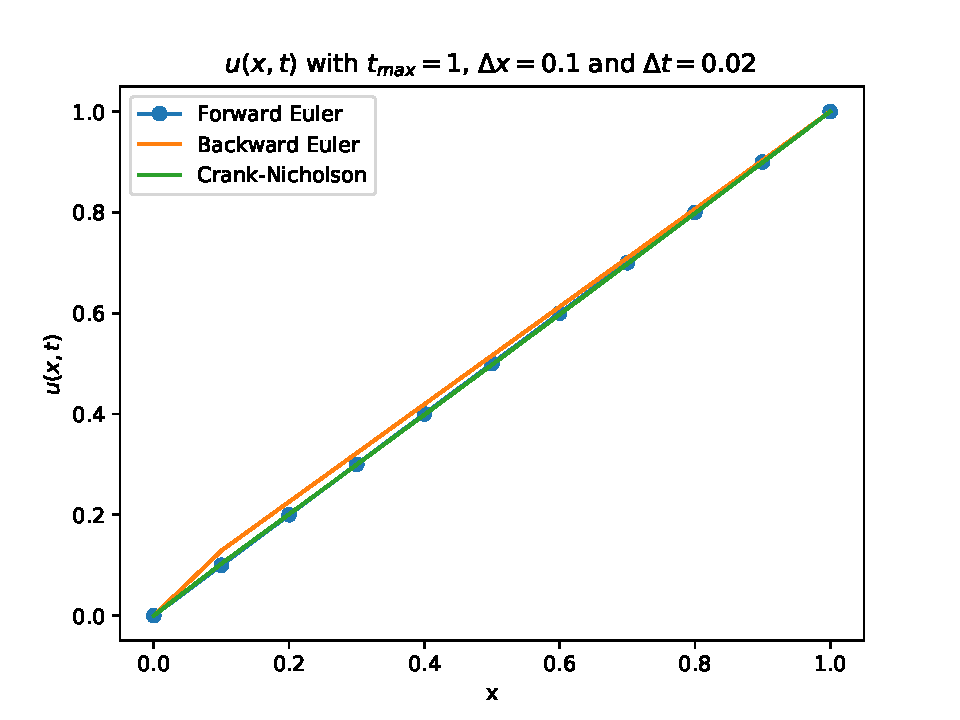
\includegraphics[width = 0.49\textwidth]{../plots/t2_10.pdf}}
  	\caption{\label{fig:methods10}Comparison of $t_1$ and $t_2$.}
\end{figure}

\begin{figure}[H]
 	\centering
  	\subfigure[\ $t_1$]{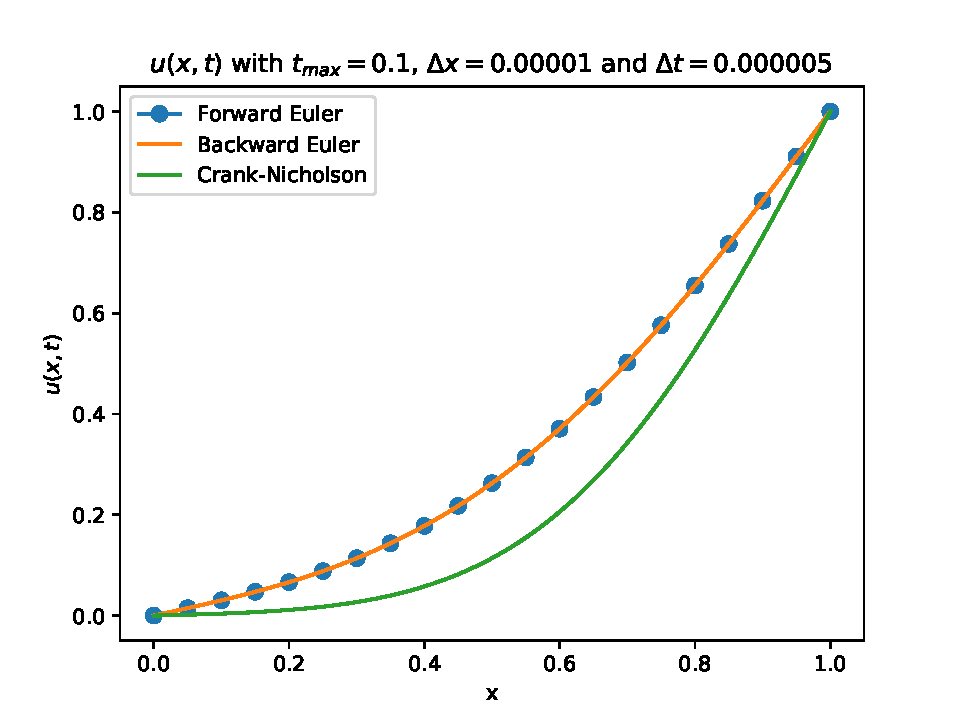
\includegraphics[width = 0.49\textwidth]{../plots/t1_100.pdf}}  
  	\subfigure[\ $t_2$]{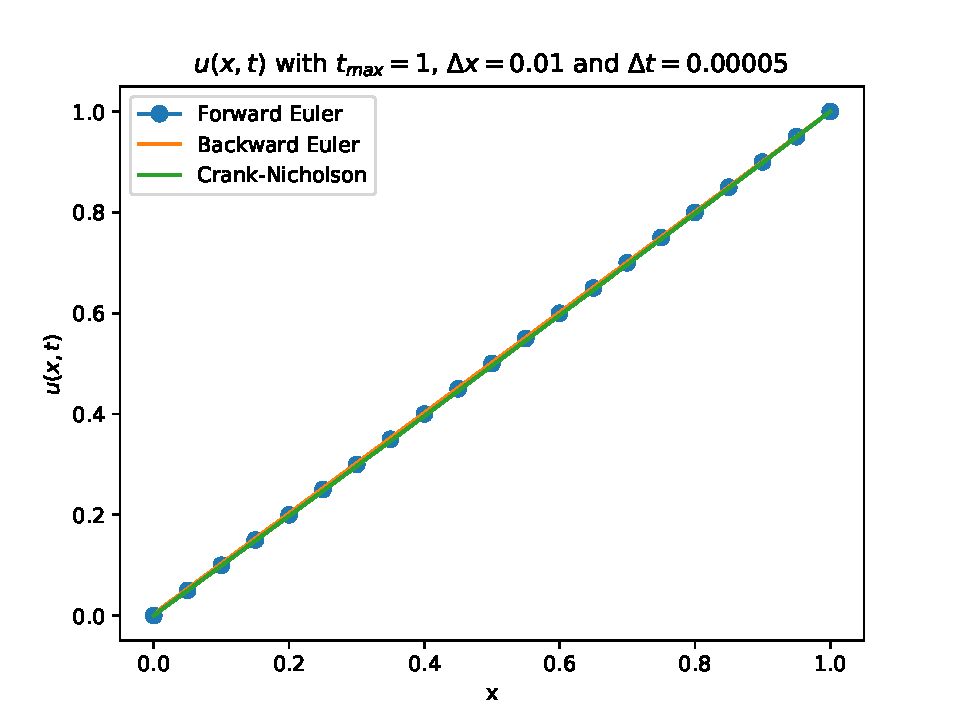
\includegraphics[width = 0.49\textwidth]{../plots/t2_100.pdf}}
  	\caption{\label{fig:methods100}Comparison of $t_1$ and $t_2$.}
\end{figure}

\noindent Figure \ref{fig:5c} highlights the distribution of temperature at two different times. At $t_1$ the different schemes produce different distributions. Forward and backward euler line up closely, in contrast to the Crank-nicolson scheme. At $t_2$ the temperature distribution is linear and all the schemes line up closely. 

\begin{figure} [H]
	\centering
	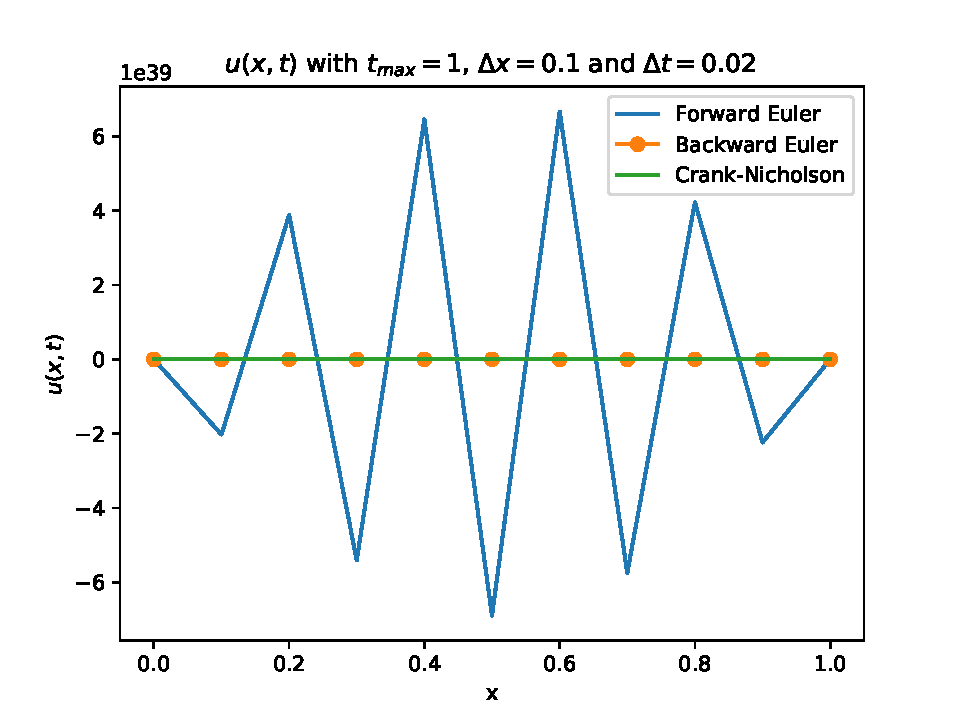
\includegraphics[width=0.48\textwidth]{../plots/unstable.pdf}
	\caption{\label{fig:unstable} Plot showing the effect of choosing unfavorable $\Delta x$ and $\Delta t$}
\end{figure}

\noindent As can be read out of Table \ref{truncstab}, the forward Euler scheme has a rigorous stability condition. Figure \ref{fig:unstable} shows a graphical representation of what happens when this condition is violated. 

\begin{figure} [H]
	\centering
	\subfigure[\ No periodic boundary conditions] {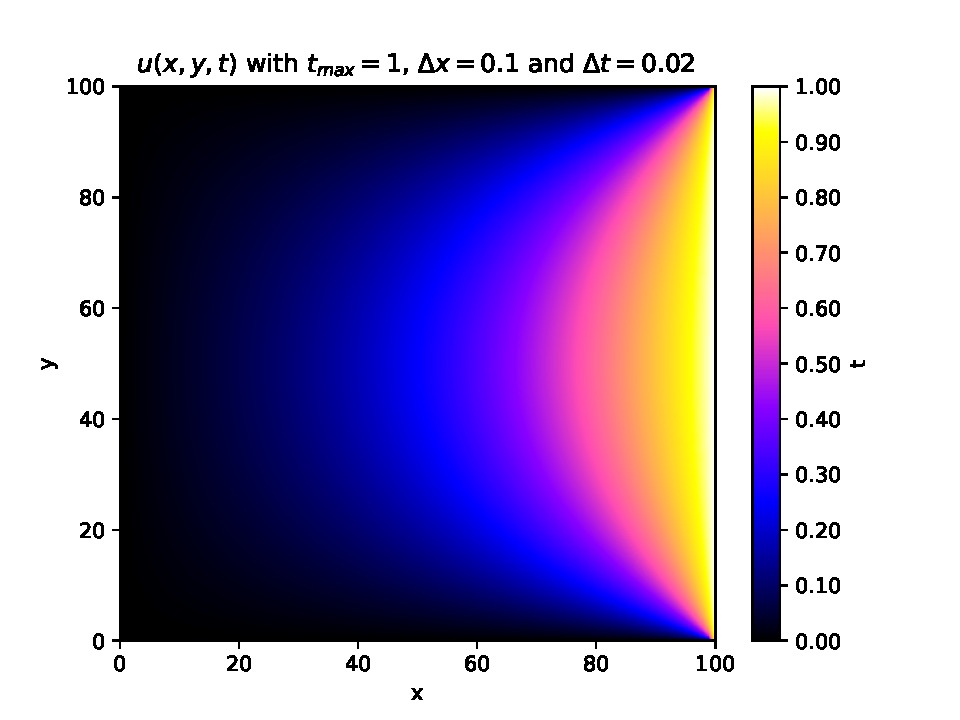
\includegraphics[width=0.48\textwidth]{../plots/bonded2D.pdf}}
	\subfigure[\ Periodic boundary conditions]{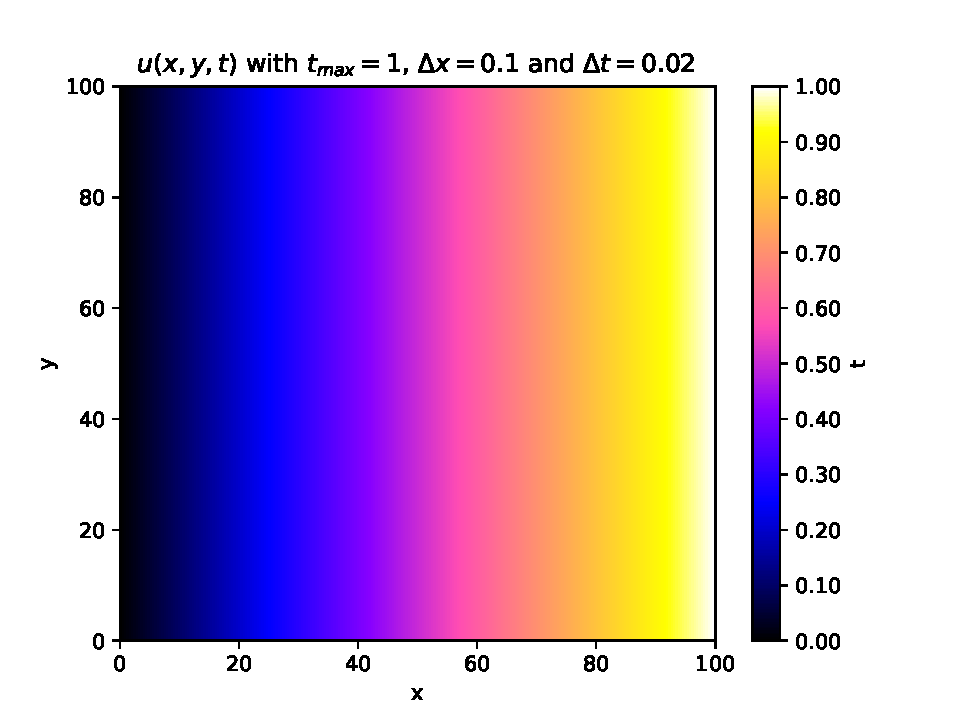
\includegraphics[width=0.48\textwidth]{../plots/periodic2D.pdf}}
	\caption{\label{fig:5d} Numerically computed two dimensional simulation with and without periodic boundary conditions}
\end{figure}

\noindent With periodic boundary conditions, the plot is giving the same result as in the one dimensional case (Figure \ref{fig:methods100}B and Figure \ref{fig:5d}B). In other words, it is showing a uniform increase in temperature with increasing $x$. Without periodic boundary conditions, there is heat loss at ell the edges except the edge with the heat source. 

\begin{figure} [H]
	\centering
	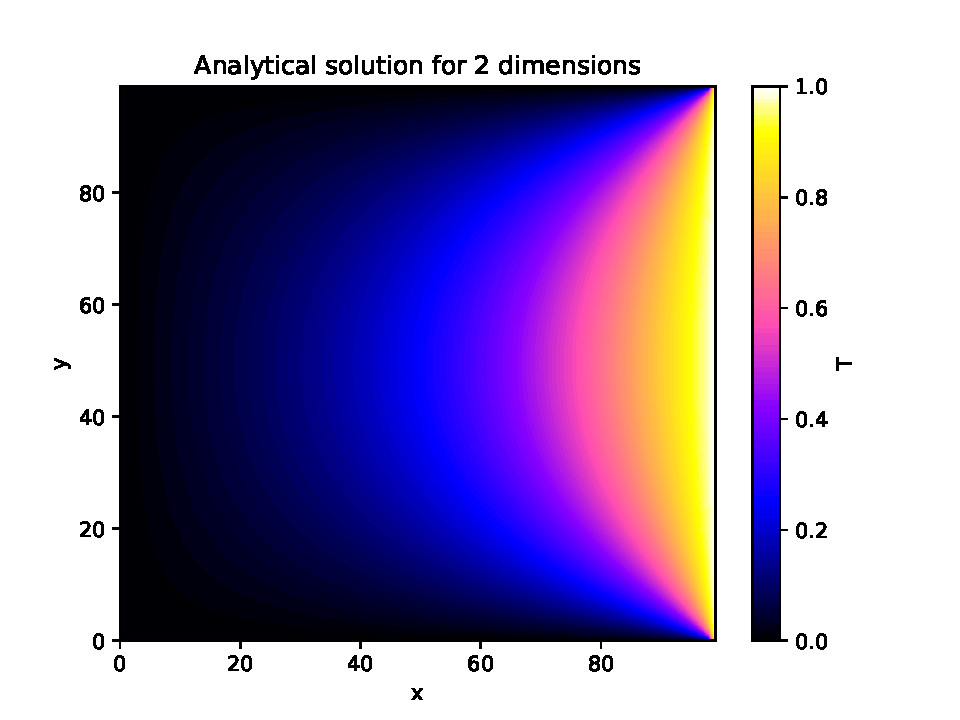
\includegraphics[width=0.48\textwidth]{../plots/2Danal.pdf}
	\caption{\label{fig:2danal} Plot showing the analytic for the two dimensional case}
\end{figure}




\begin{figure} [H]
	\centering
	\subfigure[\ ] {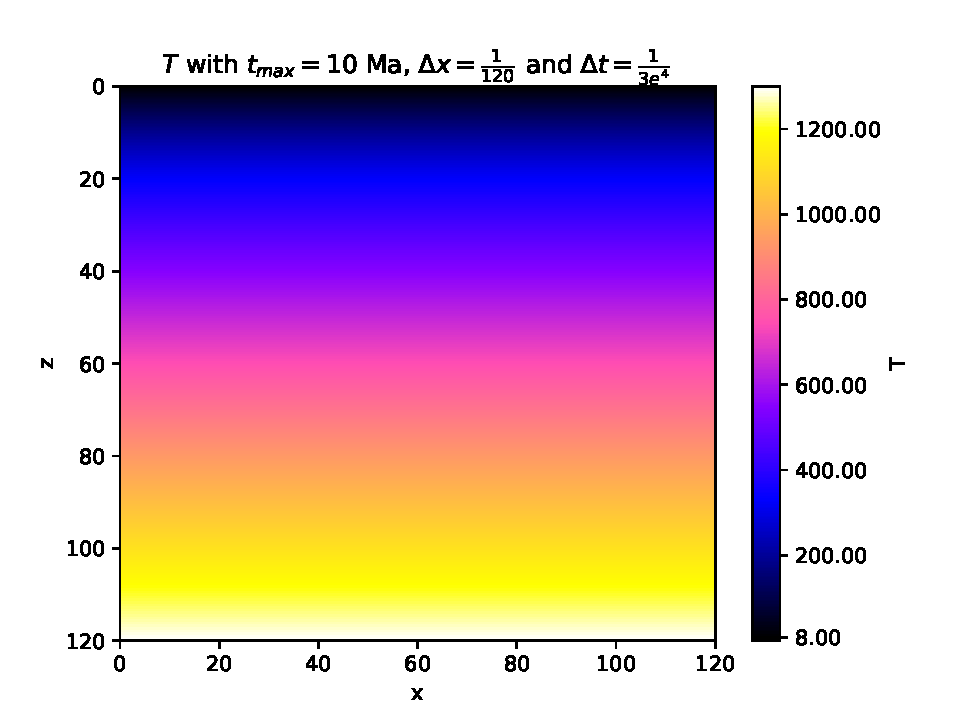
\includegraphics[width=0.48\textwidth]{../plots/contq10ma.pdf}}
	\subfigure[\ ]{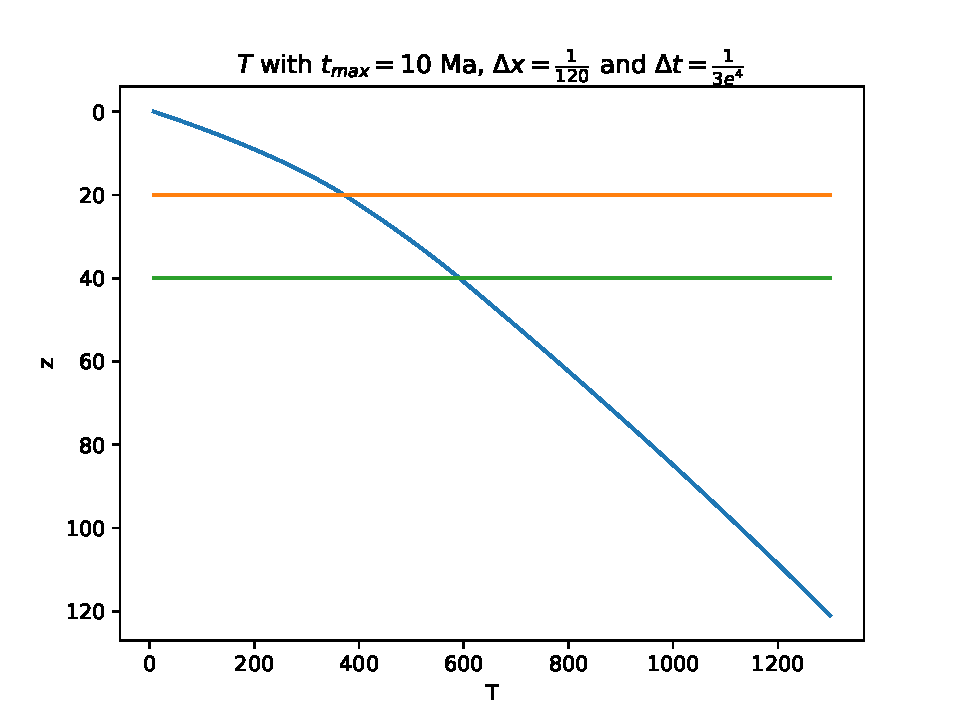
\includegraphics[width=0.48\textwidth]{../plots/lineq10ma.pdf}}
	\caption{\label{10notenriched}Numerically computed temperature distribution in the three layered lithosphere model after 10 million years, plotted in one and two dimensions without radioactive enrichment. }
\end{figure}





\begin{figure} [H]
	\centering
	\subfigure[\ ] {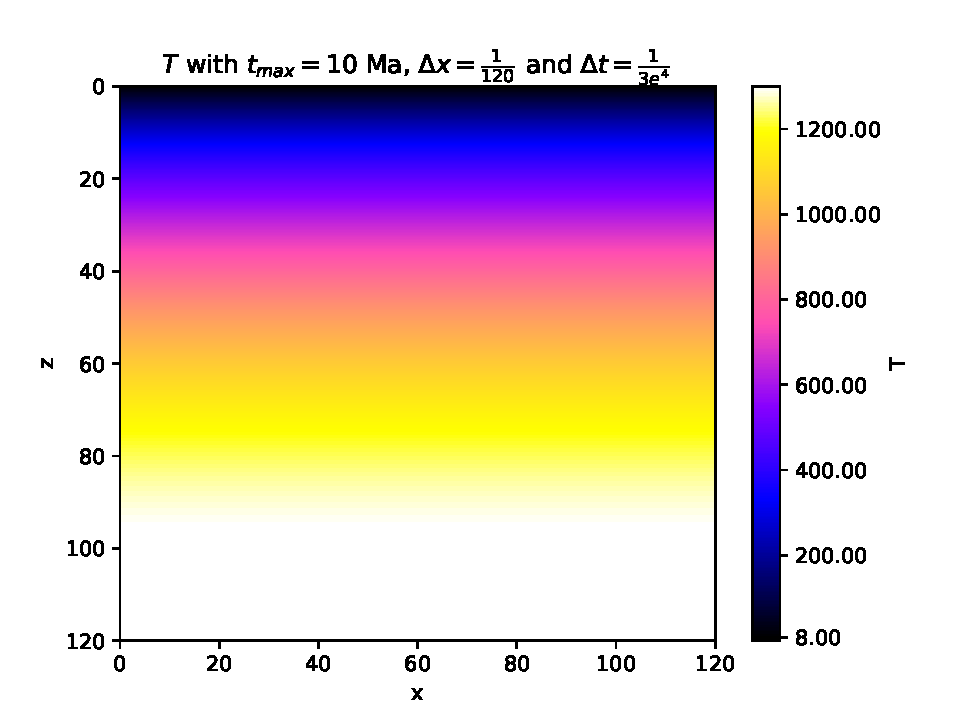
\includegraphics[width=0.48\textwidth]{../plots/contheat10ma.pdf}}
	\subfigure[\ ]{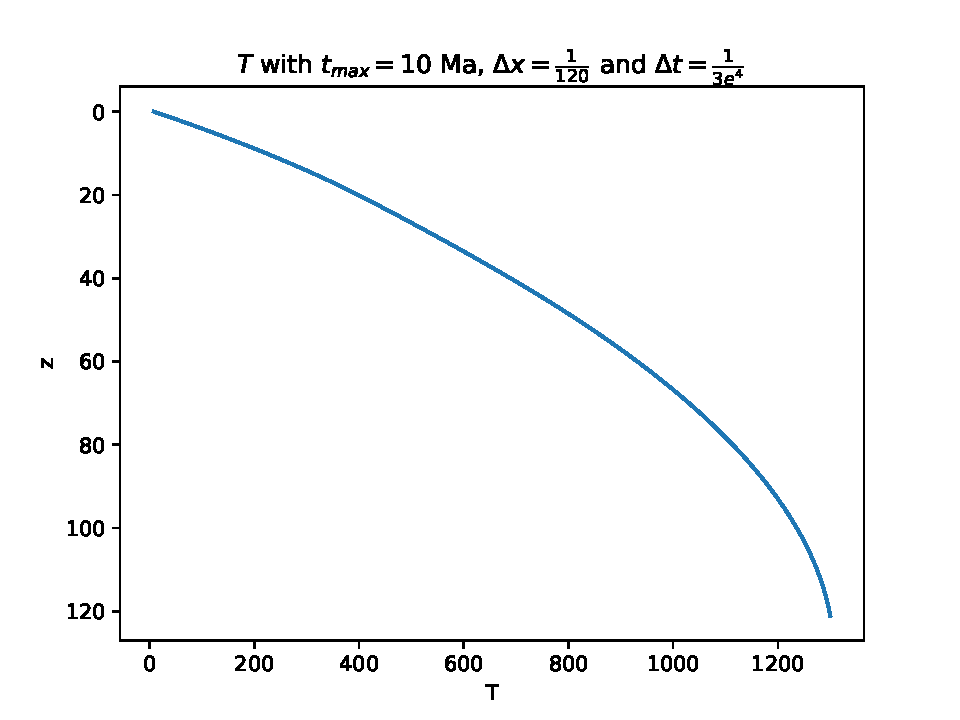
\includegraphics[width=0.48\textwidth]{../plots/lineheat10ma.pdf}}
	\caption{\label{10enriched}Numerically computed temperature distribution in the three layered lithosphere model after 10 million years, plotted in one and two dimensions with radioactive enrichment. }
\end{figure}


\noindent By using the relations described in equation $robinergay$, the $c-$values for the analytic expression can be evaluated to be:

\begin{equation}
c=\begin{bmatrix}
8\\
92\\
44\\
\end{bmatrix}\\
\vspace{0.5cm}
\end{equation}
The bottom boundary condition is used to evaluate the $b-$values. As$T_3(-120)=1300$, $c-$values are known, and $b_1,b_2$ are expressed with regard to $b_3$ (equation $robinerfortsattgay$), the $b-$values are easy to find.

\begin{equation}
b=\begin{bmatrix}
-29\\
-20.6\\
-23.8\\
\end{bmatrix}
\end{equation}
These values have been used in combination with equation $robinergay2$ to plot the analytic temperature distribution for the three layered lithosphere model (\ref{10analytic}). 


\begin{figure} [H]
	\centering
	\subfigure[\ ] {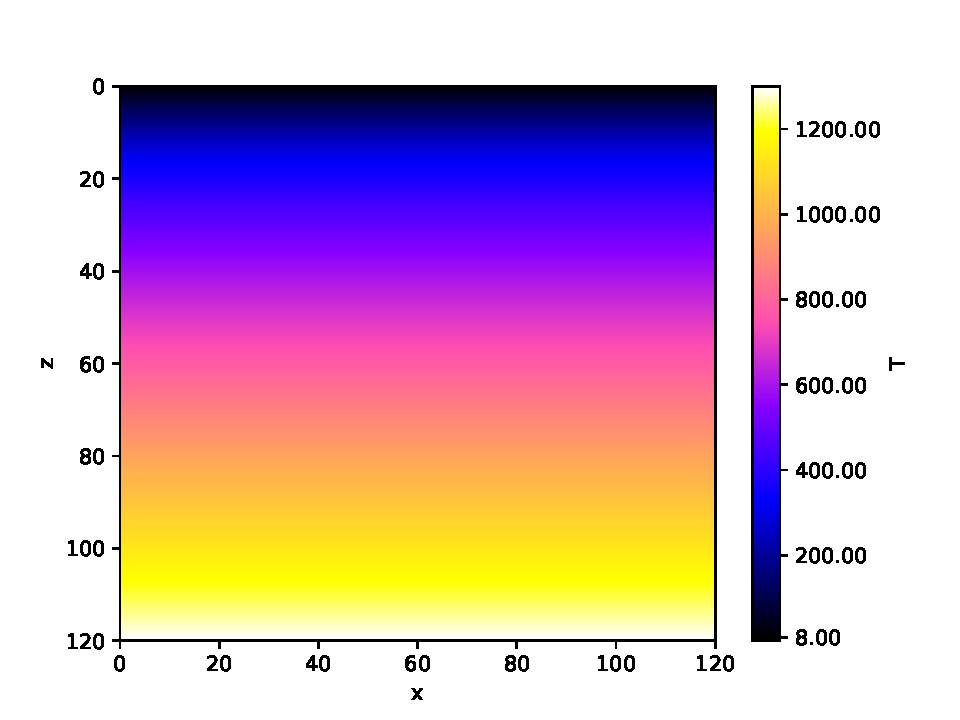
\includegraphics[width=0.48\textwidth]{../plots/contanalnorich.pdf}}
	\subfigure[\ ]{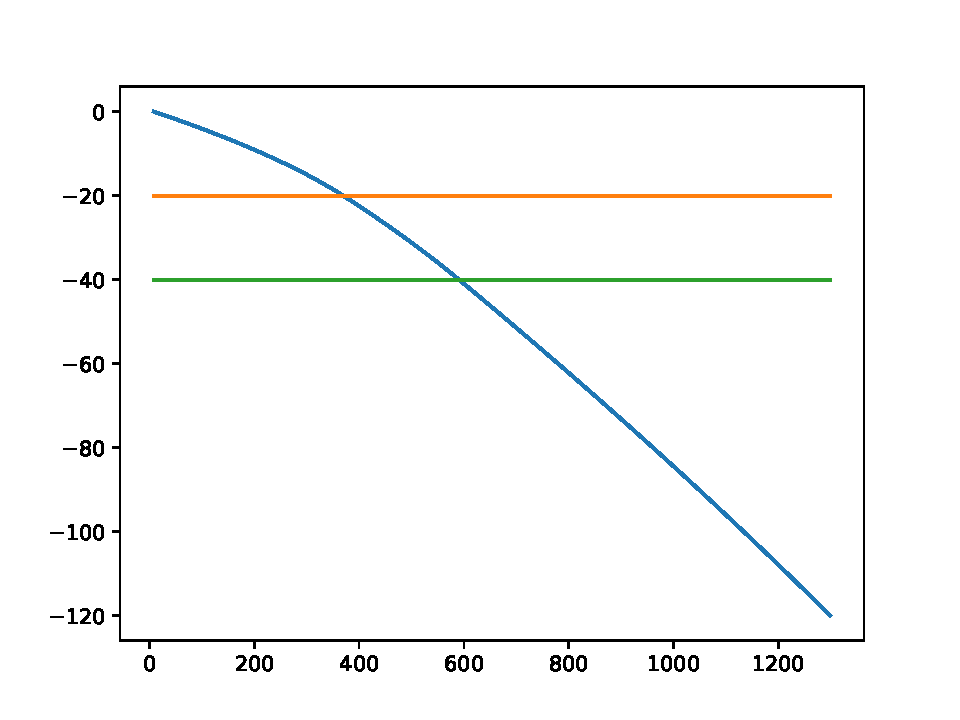
\includegraphics[width=0.48\textwidth]{../plots/lineanalnorich.pdf}}
	\caption{\label{10analyticNotEnriched}Analytic solution for the three layered lithosphere model after reaching equilibrium, plotted for one and two dimensions without radioactive enrichment. }
\end{figure}

\begin{figure} [H]
	\centering
	\subfigure[\ ] {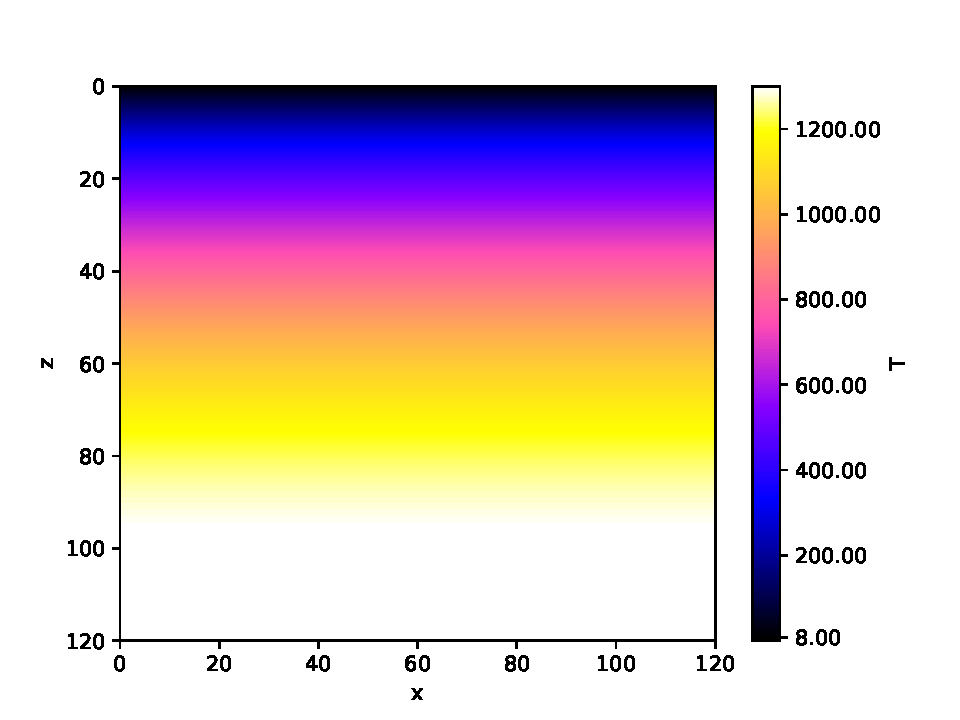
\includegraphics[width=0.48\textwidth]{../plots/contanal.pdf}}
	\subfigure[\ ]{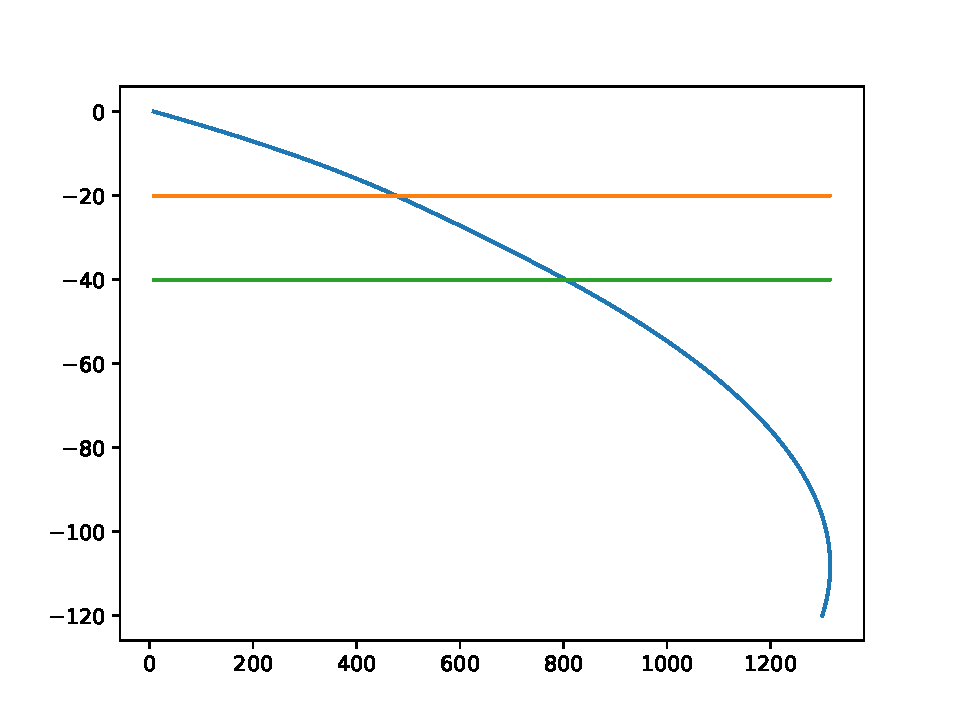
\includegraphics[width=0.48\textwidth]{../plots/lineanal.pdf}}
	\caption{\label{10analyticEnriched}Analytic solution for the three layered lithosphere model after reaching equilibrium, plotted for one and two dimensions with radioactive enrichment. }
\end{figure}



\begin{table} [H]
\centering
\caption{\% of different radioactive materials left after 1 Gy}
\begin{tabular}{|c|c|c|c|}
\hline
Radioactive material & Half-life & \% Before simulation & \% after 1 Gy\\
\hline
Potassium ($K$) 	 & 1,25 Gy   & 20 \% 				 & 11,49 \% \\
\hline
Uranium ($U$)	     & 4,47 Gy   & 40 \%				 & 34,25 \% \\
\hline
Thorium ($Th$)		 & 14,0 Gy	 & 40 \%				 & 38,07 \% \\
\hline
Sum					 & 			 & 100 \% 				 & 84.44 \%\\
\hline
\end{tabular}
\label{Decay}
\end{table}

\noindent Table \ref{Decay} is showing that a lot of the radioactive material is present even one billion years after the enrichment. The $Q$-value (heat production) before and after enrichment for the mantle is respectively $0,05$ and $0,55$. After one billion years $Q_{1Gy}=0.46442$, which is not a big reduction considering the vast time span.   

\newpage
\section*{Discussion}

Table \ref{truncstab} shows that, even though the Euler forward method is easy to implement, there are serious limitations for the stability. The Euler backward and Crank-nicolson schemes are stable for all $\Delta x$ and $\Delta t$, but the implementation is more complicated. As the euler forward and Crank-nicolson uses a tridiagonal solver in the computation process, it is expected to be slower than the Euler forward scheme, which uses a more direct approach. Figure \ref{fig:unstable} shows that the forward Euler fluctuates a lot when the stability condition is violated. The stable schemes actually produce correct results, but are drowned by the fluctuations of the forward Euler. 
\\

\noindent In the one dimensional case, the system converges to an equilibrium. This is shown graphical in figure \ref{fig:methods10} and \ref{fig:methods100}. When decreasing the $\Delta x$ and $\Delta t$, the graphs become noticeably smoother. Moreover, the errors decrease in accordance with Table \ref{truncstab}. It is hard to compare the three schemes in terms of quality. The explicit scheme is unstable for some values (Table \ref{truncstab}, Figure \ref{fig:unstable}), but is easy to implement and computing efficient. The implicit Euler backward scheme is less computing efficient than the explicit scheme, but does not suffer from the same stability limitations. The Crank-Nicolson scheme is stable for all $\Delta t$ and $\Delta x$ and has the smallest truncation error when $\Delta t$ is small, but has its drawback in computing efficiency. On account of the above mentioned properties, it is impossible to unambiguously decide which scheme is best. Each has its advantages and drawbacks, and the most favorable scheme depends heavily on what is to be computed.\\

\noindent Given the boundary conditions $u(0,t)=0$ and $u(1,t)=1$ for all $t$, this can be translated to a one dimensional rod with  a heat source at $x=1$ and a heat sink at $x=0$. When starting the computation, the only point with a nonzero temperature is at $x=1$. The heat from this point then spreads through the rod. The heat rises quicker close to the heat source, as is shown in figure \ref{fig:methods10}A and \ref{fig:methods100}A, but will with time reach an equilibrium (figure \ref{fig:methods10}B,\ref{fig:methods100}B). It is important to note that the behavior of the system is entirely dependent on the boundary conditions. As an example, it would be possible to add another heat source at $x=0$ and the temperature would rise from both edges.   
\\

\noindent The boundary conditions in the two dimensional case depends on what kind of system being simulated. If the system in question is a two dimensional rod with a heat source at one end and heat loss at all the other edges, the temperature distribution would look like figure \ref{fig:5d}A or figure \ref{fig:2danal}. If the system is for the temperature distribution in the lithosphere, it is not expected to be much heat loss in the lateral direction. This can be simulated with periodic boundary conditions, which in essence removes all lateral heat loss. 
\\

\noindent The last case looked on is the three layered lithosphere model. This was solved in two dimensions, and with a size of $120 \times 120$ km. The focus was put on the vertical temperature distribution. The model was simulated using periodic boundary conditions and using the forward euler method. To run the code, and get a reasonable result within the time limit, all the constants had to be rescaled. Without scaling, it would have been impossible to get stable results for larger time spans.   



\noindent Without any heat production, the temperature distribution would be a linearly dependent on depth. As the three layers have varying heat production, the distribution will not be linear. The larger amount of radioactive material in the crust results in a larger temperature increase in this layer. This can be read directly from the heat production, and is also mirrored in the plots representing temperature distribution before radioactive enrichment (Figure \ref{10notenriched}).\\ 


\noindent After radioactive enrichment, the heat production of the mantle is altered. This increases the temperature in the bottom layer, which in turn increase the temperature throughout the entire model (Figure \ref{10enriched},\ref{10analytic}). The radioactive material consists of three different materials with different half-lives (Table \ref{Decay}). As stated earlier, the reduction of radioactive material is small compared to the time span Table \ref{Decay}). On account of this, it is a good approximation to disregard this effect.  



\newpage
\section*{Concluding remarks}
Three algorithms have been used in this project, each having different drawbacks and advantages. The explicit forward Euler scheme is efficient and easy to implement, but has a rigorous stability condition for step size. The implicit Euler backward is stable for all step sizes, but is less efficient, as it uses a tridiagonal solver in the computation process. The Crank-Nicolson scheme is stable for all step sizes in addition to providing the smallest truncation error of the schemes. The drawback of this method is somewhat similar to the Euler backward scheme, as both use a tridiagonal solver.\\ 

\noindent The idealized one dimensional case showed that the all the three algorithms quickly converge to an equilibrium. The result of the two dimensional case is entirely dependent on the choice of boundary conditions. With periodic boundary conditions, it creates a homogeneous increase in temperature with increasing x. The three layered lithosphere was modeled with random boundary conditions. The biggest difference before and after radioactive enrichment is that the temperature is higher throughout the model. In addition, the temperature distribution in the mantle goes from being approximately linear, to being curved.  




\newpage
\section*{References}


\end{document}
